%%%%%%%%%%%%  Generated using docx2latex.com  %%%%%%%%%%%%%%

%%%%%%%%%%%%  v2.0.0-beta  %%%%%%%%%%%%%%

\documentclass[12pt]{article}
\usepackage{amsmath}
\usepackage{latexsym}
\usepackage{amsfonts}
\usepackage[normalem]{ulem}
\usepackage{array}
\usepackage{amssymb}
\usepackage{graphicx}
\usepackage[backend=biber,
style=numeric,
sorting=none,
isbn=false,
doi=false,
url=false,
]{biblatex}\addbibresource{bibliography.bib}

\usepackage{subfig}
\usepackage{wrapfig}
\usepackage{wasysym}
\usepackage{enumitem}
\usepackage{adjustbox}
\usepackage{ragged2e}
\usepackage[svgnames,table]{xcolor}
\usepackage{tikz}
\usepackage{longtable}
\usepackage{changepage}
\usepackage{setspace}
\usepackage{hhline}
\usepackage{multicol}
\usepackage{tabto}
\usepackage{float}
\usepackage{multirow}
\usepackage{makecell}
\usepackage{fancyhdr}
\usepackage[toc,page]{appendix}
\usepackage[hidelinks]{hyperref}
\usetikzlibrary{shapes.symbols,shapes.geometric,shadows,arrows.meta}
\tikzset{>={Latex[width=1.5mm,length=2mm]}}
\usepackage{flowchart}\usepackage[paperheight=11.0in,paperwidth=8.5in,left=0.79in,right=0.79in,top=0.79in,bottom=0.79in,headheight=1in]{geometry}
\usepackage[utf8]{inputenc}
\usepackage[T1]{fontenc}
\TabPositions{0.49in,0.98in,1.47in,1.96in,2.45in,2.94in,3.43in,3.92in,4.41in,4.9in,5.39in,5.88in,6.37in,6.86in,}

\urlstyle{same}


 %%%%%%%%%%%%  Set Depths for Sections  %%%%%%%%%%%%%%

% 1) Section
% 1.1) SubSection
% 1.1.1) SubSubSection
% 1.1.1.1) Paragraph
% 1.1.1.1.1) Subparagraph


\setcounter{tocdepth}{5}
\setcounter{secnumdepth}{5}


 %%%%%%%%%%%%  Set Depths for Nested Lists created by \begin{enumerate}  %%%%%%%%%%%%%%


\setlistdepth{9}
\renewlist{enumerate}{enumerate}{9}
		\setlist[enumerate,1]{label=\arabic*)}
		\setlist[enumerate,2]{label=\alph*)}
		\setlist[enumerate,3]{label=(\roman*)}
		\setlist[enumerate,4]{label=(\arabic*)}
		\setlist[enumerate,5]{label=(\Alph*)}
		\setlist[enumerate,6]{label=(\Roman*)}
		\setlist[enumerate,7]{label=\arabic*}
		\setlist[enumerate,8]{label=\alph*}
		\setlist[enumerate,9]{label=\roman*}

\renewlist{itemize}{itemize}{9}
		\setlist[itemize]{label=$\cdot$}
		\setlist[itemize,1]{label=\textbullet}
		\setlist[itemize,2]{label=$\circ$}
		\setlist[itemize,3]{label=$\ast$}
		\setlist[itemize,4]{label=$\dagger$}
		\setlist[itemize,5]{label=$\triangleright$}
		\setlist[itemize,6]{label=$\bigstar$}
		\setlist[itemize,7]{label=$\blacklozenge$}
		\setlist[itemize,8]{label=$\prime$}

\setlength{\topsep}{0pt}\setlength{\parindent}{0pt}
\renewcommand{\arraystretch}{1.3}


%%%%%%%%%%%%%%%%%%%% Document code starts here %%%%%%%%%%%%%%%%%%%%



\begin{document}
\setlength{\parskip}{6.0pt}
{\fontsize{18pt}{21.6pt}\selectfont \textbf{ARREGLOS Y PARÁMETROS DE LOS AMPLIFICADORES CLASE B}\par}\par

\textbf{POR: Jesús David Esparza Cabrera}\par


\vspace{\baselineskip}
{\fontsize{18pt}{21.6pt}\selectfont \textbf{ INTRODUCCIÓN}\par}\par

Un amplificador recibe una señal de algún transductor de \href{https://www.monografias.com/trabajos/adpreclu/adpreclu.shtml}{capacitación} o de cualquier otra fuente de entrada y proporciona una versión más grande de la señal a cierto dispositivo de salida o a otra etapa de amplificación.\par

Un amplificador de voltaje amplificación de voltaje principalmente para incrementar voltaje de la señal de entrada, Por otro lado, los amplificadores de gran señal o de \href{https://www.monografias.com/trabajos14/trmnpot/trmnpot.shtml}{potencia}, proporcionan principalmente potencia suficiente a una carga de salida para activar una bocina o algún otro dispositivo.\par

Es decir un amplificador de potencia es aquel que, aparte de suministrar una mayor tensión, suministran también una mayor \href{http://www.unicrom.com/Tut_corriente_electrica.asp}{corriente }(amplificación de tensión y amplificación de corriente y, por ende, amplificación de potencia).\par

En este tema únicamente vamos a entrar en los amplificadores de potencia \href{https://www.monografias.com/trabajos901/debate-multicultural-etnia-clase-nacion/debate-multicultural-etnia-clase-nacion.shtml}{clase} b, que son los que nos interesan.\par

{\fontsize{18pt}{21.6pt}\selectfont \textbf{II \href{https://www.monografias.com/trabajos12/desorgan/desorgan.shtml}{DESARROLLO} DE LOS CONTENIDOS}\par}\par

\begin{itemize}
	\item \textbf{A. PRINCIPIO DE FUNCIONAMIENTO DE UN AMPLIFICADOR DE POTENCIA CLASE B}
\end{itemize}\par

Un amplificador de potencia funciona en clase B cuando la polarización de dc deja al \href{https://www.monografias.com/trabajos11/trans/trans.shtml}{transistor} casi apagado de manera que el transistor se enciende cuando a este se le aplica una señal en ac. Es decir que le transistor conducirá corriente solamente para una mitad de ciclo de la señal.\par

Ahora para obtener una señal de ciclo completo será necesario utilizar dos \href{https://www.monografias.com/trabajos11/trans/trans.shtml}{transistores} y lograr que cada uno de ellos conduzca durante \href{https://www.monografias.com/trabajos14/medios-comunicacion/medios-comunicacion.shtml}{medios} ciclos opuestos, y al tener esta operación combinada se obtiene un ciclo completo de señal de salida.\par

Dado que una parte del circuito "empuja" a la señal de arriba durante una mitad del ciclo y la otra parte "jala" la señal hacia abajo durante la otra mitad del ciclo, el circuito por ende se denomina de contrafase circuito push-pull.\par



%%%%%%%%%%%%%%%%%%%% Figure/Image No: 1 starts here %%%%%%%%%%%%%%%%%%%%

\begin{figure}[H]
	\begin{Center}
		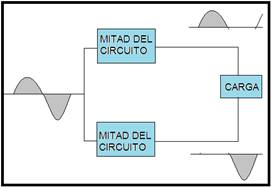
\includegraphics[width=2.82in,height=1.95in]{./media/image1.jpeg}
	\end{Center}
\end{figure}


%%%%%%%%%%%%%%%%%%%% Figure/Image No: 1 Ends here %%%%%%%%%%%%%%%%%%%%

\par

\textbf{FIGURA 1}. Representación en bloques de la operación en contrafase\par

Los transistores de potencia empleados en el circuito de contrafase son capaces de entregar la potencia deseada a la carga, y la operación clase B de estos transistores proporciona una diferencia mayor que la que era posible mediante un solo transistor en la operación clase A.\par



%%%%%%%%%%%%%%%%%%%% Figure/Image No: 2 starts here %%%%%%%%%%%%%%%%%%%%

\begin{figure}[H]
	\begin{Center}
		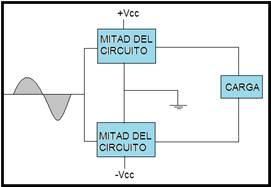
\includegraphics[width=2.82in,height=1.95in]{./media/image2.jpeg}
	\end{Center}
\end{figure}


%%%%%%%%%%%%%%%%%%%% Figure/Image No: 2 Ends here %%%%%%%%%%%%%%%%%%%%

\par

\textbf{FIGURA 2}. Conexión del amplificador en contrafase con la carga mediante dos fuentes de voltaje.\par



%%%%%%%%%%%%%%%%%%%% Figure/Image No: 3 starts here %%%%%%%%%%%%%%%%%%%%

\begin{figure}[H]
	\begin{Center}
		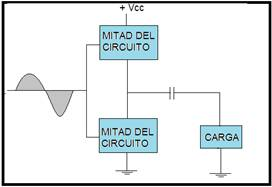
\includegraphics[width=2.83in,height=1.95in]{./media/image3.jpeg}
	\end{Center}
\end{figure}


%%%%%%%%%%%%%%%%%%%% Figure/Image No: 3 Ends here %%%%%%%%%%%%%%%%%%%%

\par

\textbf{FIGURA 3}. Conexión del amplificador en contrafase con la carga mediante una fuente de voltaje.\par

\begin{itemize}
	\item \textbf{B. ANALISIS EN DC}
\end{itemize}\par



%%%%%%%%%%%%%%%%%%%% Figure/Image No: 4 starts here %%%%%%%%%%%%%%%%%%%%

\begin{figure}[H]
	\begin{Center}
		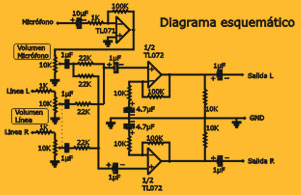
\includegraphics[width=2.81in,height=2.1in]{./media/image4.gif}
	\end{Center}
\end{figure}


%%%%%%%%%%%%%%%%%%%% Figure/Image No: 4 Ends here %%%%%%%%%%%%%%%%%%%%

\par

\textbf{FIGURA 4.} Circuito completo \par



%%%%%%%%%%%%%%%%%%%% Figure/Image No: 5 starts here %%%%%%%%%%%%%%%%%%%%

\begin{figure}[H]
	\begin{Center}
		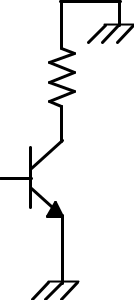
\includegraphics[width=2.25in,height=2.12in]{./media/image5.gif}
	\end{Center}
\end{figure}


%%%%%%%%%%%%%%%%%%%% Figure/Image No: 5 Ends here %%%%%%%%%%%%%%%%%%%%

\par

\textbf{FIGURA 5.} Circuito equivalente para continua\par



%%%%%%%%%%%%%%%%%%%% Figure/Image No: 6 starts here %%%%%%%%%%%%%%%%%%%%

\begin{figure}[H]
	\begin{Center}
		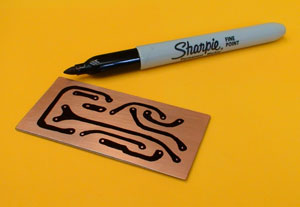
\includegraphics[width=0.44in,height=0.15in]{./media/image6.gif}
	\end{Center}
\end{figure}


%%%%%%%%%%%%%%%%%%%% Figure/Image No: 6 Ends here %%%%%%%%%%%%%%%%%%%%

Con el circuito expuesto en la figura 5 se comienza el análisis en continua, el diseñador selecciona las resistencias de polarización para definir el punto Q en el corte. Esto polariza el diodo emisor de cada transistor entre 0,6 y 0,7 V de modo que estén al borde la conducción idealmente \par

Puesto que las resistencias de polarización son iguales, cada diodo emisor se polariza con el mismo \href{https://www.monografias.com/trabajos14/nuevmicro/nuevmicro.shtml}{valor} de tensión, como resultado, la mitad de \href{https://www.monografias.com/Salud/Nutricion/}{alimentación} cae en los terminales colector- emisor de cada transistor. Es decir\par



%%%%%%%%%%%%%%%%%%%% Figure/Image No: 7 starts here %%%%%%%%%%%%%%%%%%%%

\begin{figure}[H]
	\begin{Center}
		
\includegraphics[width=0.65in,height=0.3in]{./media/image7.gif}
	\end{Center}
\end{figure}


%%%%%%%%%%%%%%%%%%%% Figure/Image No: 7 Ends here %%%%%%%%%%%%%%%%%%%%

\par

\textbf{B.1. RECTA DE CARGA EN CONTINUA}\par

Debido a que no existe ninguna \href{https://www.monografias.com/trabajos10/restat/restat.shtml}{resistencia} en los circuitos de colector ni de emisor como se observa en la figura 5, la corriente continua de saturación es infinita. Esto significa que la recta de carga continua es vertical .Lo mas complicado en el \href{https://www.monografias.com/trabajos13/diseprod/diseprod.shtml}{diseño} de los amplificadores clase B es configurar un punto Q estable en la región de corte.\par

\textbf{B.2}. \textbf{RECTA DE CARGA EN ALTERNA}\par

Cuando cualquiera de los transistores esta conduciendo, su punto de operación se desplaza a lo largo de la recta de carga en alterna. La amplitud de la tensión del transistor que está en conducción puede variar entre el corte y la saturación. En el otro semiciclo, el otro transistor tendrá este mismo \href{https://www.monografias.com/trabajos16/comportamiento-humano/comportamiento-humano.shtml}{comportamiento}. Esto significa que la salida máxima pico a pico es:\par



%%%%%%%%%%%%%%%%%%%% Figure/Image No: 8 starts here %%%%%%%%%%%%%%%%%%%%

\begin{figure}[H]
	\begin{Center}
		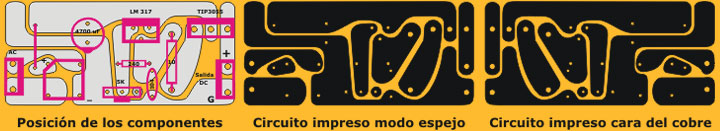
\includegraphics[width=0.69in,height=0.09in]{./media/image8.gif}
	\end{Center}
\end{figure}


%%%%%%%%%%%%%%%%%%%% Figure/Image No: 8 Ends here %%%%%%%%%%%%%%%%%%%%

\par



%%%%%%%%%%%%%%%%%%%% Figure/Image No: 9 starts here %%%%%%%%%%%%%%%%%%%%

\begin{figure}[H]
	\begin{Center}
		
\includegraphics[width=2.81in,height=2.27in]{./media/image9.gif}
	\end{Center}
\end{figure}


%%%%%%%%%%%%%%%%%%%% Figure/Image No: 9 Ends here %%%%%%%%%%%%%%%%%%%%

\par

\textbf{FIGURA 6.} Rectas de carga en continua y alterna\par

\begin{itemize}
	\item \textbf{C. ANALISIS EN AC}
\end{itemize}\par



%%%%%%%%%%%%%%%%%%%% Figure/Image No: 10 starts here %%%%%%%%%%%%%%%%%%%%

\begin{figure}[H]
	\begin{Center}
		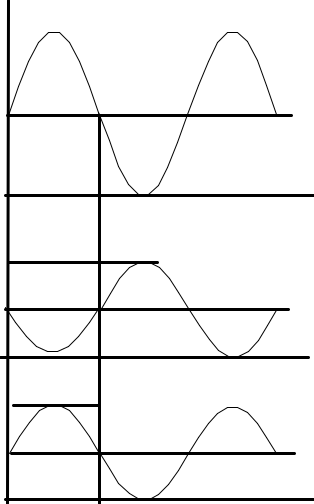
\includegraphics[width=2.81in,height=1.82in]{./media/image10.gif}
	\end{Center}
\end{figure}


%%%%%%%%%%%%%%%%%%%% Figure/Image No: 10 Ends here %%%%%%%%%%%%%%%%%%%%

\par

\textbf{FIGURA 7.} Circuito equivalente en alterna\par

Como se \href{https://www.monografias.com/trabajos11/tebas/tebas.shtml}{muestra} en la figura 7 el circuito equivalente en alterna del transistor el mismo esta conduciendo. Ignorando re la ganancia de tensión es:\par



%%%%%%%%%%%%%%%%%%%% Figure/Image No: 11 starts here %%%%%%%%%%%%%%%%%%%%

\begin{figure}[H]
	\begin{Center}
		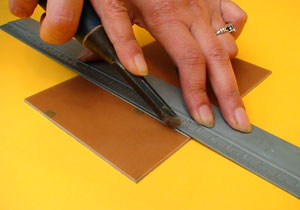
\includegraphics[width=0.42in,height=0.12in]{./media/image11.gif}
	\end{Center}
\end{figure}


%%%%%%%%%%%%%%%%%%%% Figure/Image No: 11 Ends here %%%%%%%%%%%%%%%%%%%%

\par

Y la impedancia de entrada de la base es:\par



%%%%%%%%%%%%%%%%%%%% Figure/Image No: 12 starts here %%%%%%%%%%%%%%%%%%%%

\begin{figure}[H]
	\begin{Center}
		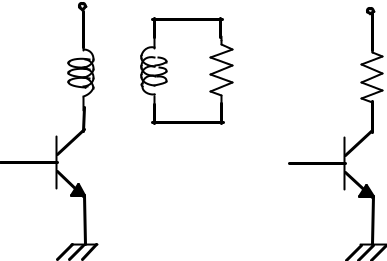
\includegraphics[width=0.92in,height=0.15in]{./media/image12.gif}
	\end{Center}
\end{figure}


%%%%%%%%%%%%%%%%%%%% Figure/Image No: 12 Ends here %%%%%%%%%%%%%%%%%%%%

\par

\begin{itemize}
	\item \textbf{D. FUNCIONAMIENTO GLOBAL}
\end{itemize}\par

En el semiciclo positivo de la tensión de entrada, el transistor superior de la figura 4 conduce y el inferior esta cortado. El transistor superior se comporta como un seguidor a emisor normal, por lo que la tensión de salida es aproximadamente igual a la tensión de entrada.\par

En el semiciclo negativo de la tensión de entrada, el transistor superior está cortado y el transistor inferior conduce. El transistor inferior se comporta como un seguidor de emisor normal y produce una tensión de carga aproximadamente igual a la tensión de entrada. El transistor superior maneja el semiciclo positivo de la tensión de entrada y el transistor inferior se ocupa del semiciclo negativo. Durante cada semiciclo, la fuente ve una alta impedancia en cualquiera de las bases.\par

\begin{itemize}
	\item \textbf{E. POTENCIA DE ENTRADA (dc)}
\end{itemize}\par

La potencia proporcionada a la carga por un amplificador se toma de la fuente de alimentación (o fuentes de alimentación) que proporciona la potencia de entrada de dc. La cantidad de esta potencia de entrada puede ser calculada mediante\par



%%%%%%%%%%%%%%%%%%%% Figure/Image No: 13 starts here %%%%%%%%%%%%%%%%%%%%

\begin{figure}[H]
	\begin{Center}
		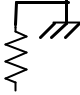
\includegraphics[width=1.26in,height=0.15in]{./media/image13.gif}
	\end{Center}
\end{figure}


%%%%%%%%%%%%%%%%%%%% Figure/Image No: 13 Ends here %%%%%%%%%%%%%%%%%%%%

\par

Donde:\par



%%%%%%%%%%%%%%%%%%%% Figure/Image No: 14 starts here %%%%%%%%%%%%%%%%%%%%

\begin{figure}[H]
	\begin{Center}
		
\includegraphics[width=1.89in,height=0.12in]{./media/image14.gif}
	\end{Center}
\end{figure}


%%%%%%%%%%%%%%%%%%%% Figure/Image No: 14 Ends here %%%%%%%%%%%%%%%%%%%%

\par



%%%%%%%%%%%%%%%%%%%% Figure/Image No: 15 starts here %%%%%%%%%%%%%%%%%%%%

\begin{figure}[H]
	\begin{Center}
		
\includegraphics[width=0.17in,height=0.12in]{./media/image15.gif}
	\end{Center}
\end{figure}


%%%%%%%%%%%%%%%%%%%% Figure/Image No: 15 Ends here %%%%%%%%%%%%%%%%%%%%

Se consume de las fuentes de alimentación. En la operación clase B, el \href{https://www.monografias.com/trabajos35/consumo-inversion/consumo-inversion.shtml}{consumo} de corriente de una sola fuente de alimentación tiene la forma de una señal rectificada de onda completa, mientras que la extraída de dos fuentes de alimentación tiene la forma de una señal rectificada demedia onda de cada fuente. Donde el valor promedio de la corriente puede expresarse de la siguiente manera.\par



%%%%%%%%%%%%%%%%%%%% Figure/Image No: 16 starts here %%%%%%%%%%%%%%%%%%%%

\begin{figure}[H]
	\begin{Center}
		
\includegraphics[width=1.25in,height=0.3in]{./media/image16.gif}
	\end{Center}
\end{figure}


%%%%%%%%%%%%%%%%%%%% Figure/Image No: 16 Ends here %%%%%%%%%%%%%%%%%%%%

\par

Donde:\par



%%%%%%%%%%%%%%%%%%%% Figure/Image No: 17 starts here %%%%%%%%%%%%%%%%%%%%

\begin{figure}[H]
	\begin{Center}
		
\includegraphics[width=2.57in,height=0.15in]{./media/image17.gif}
	\end{Center}
\end{figure}


%%%%%%%%%%%%%%%%%%%% Figure/Image No: 17 Ends here %%%%%%%%%%%%%%%%%%%%

\par



%%%%%%%%%%%%%%%%%%%% Figure/Image No: 18 starts here %%%%%%%%%%%%%%%%%%%%

\begin{figure}[H]
	\begin{Center}
		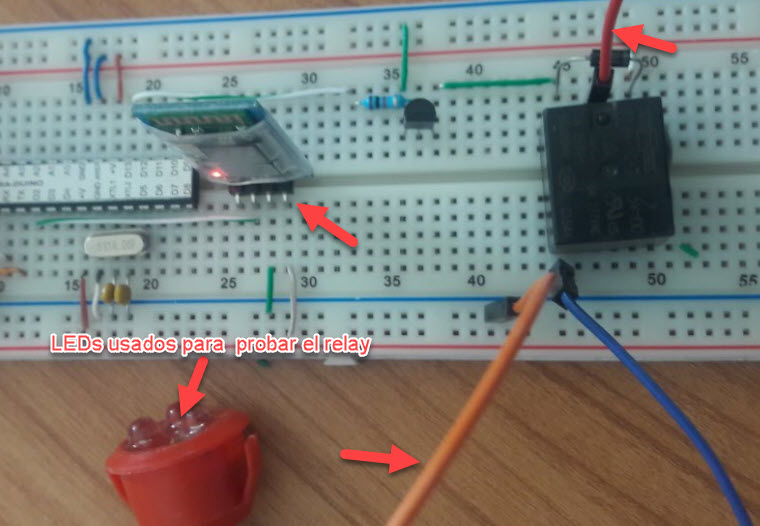
\includegraphics[width=1.34in,height=0.09in]{./media/image18.gif}
	\end{Center}
\end{figure}


%%%%%%%%%%%%%%%%%%%% Figure/Image No: 18 Ends here %%%%%%%%%%%%%%%%%%%%

\par

Al utilizar la ecuación [2] en la ecuación de potencia de entrada [1] se obtiene:\par



%%%%%%%%%%%%%%%%%%%% Figure/Image No: 19 starts here %%%%%%%%%%%%%%%%%%%%

\begin{figure}[H]
	\begin{Center}
		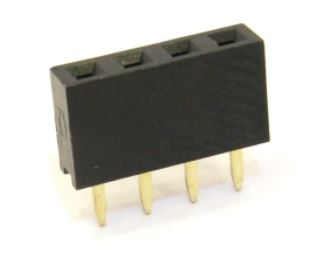
\includegraphics[width=1.74in,height=0.3in]{./media/image19.gif}
	\end{Center}
\end{figure}


%%%%%%%%%%%%%%%%%%%% Figure/Image No: 19 Ends here %%%%%%%%%%%%%%%%%%%%

\par

\begin{itemize}
	\item \textbf{F. POTENCIA DE SALIDA (ac)}
\end{itemize}\par



%%%%%%%%%%%%%%%%%%%% Figure/Image No: 20 starts here %%%%%%%%%%%%%%%%%%%%

\begin{figure}[H]
	\begin{Center}
		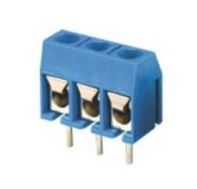
\includegraphics[width=0.14in,height=0.12in]{./media/image20.gif}
	\end{Center}
\end{figure}


%%%%%%%%%%%%%%%%%%%% Figure/Image No: 20 Ends here %%%%%%%%%%%%%%%%%%%%

La potencia aplicada a la carga (referida comúnmente como una resistencia se puede calcular mediante cualquiera de distintas ecuaciones. Si se utiliza un medidor rms para medir el voltaje a través de la carga, la potencia de salida se puede calcular como:\par



%%%%%%%%%%%%%%%%%%%% Figure/Image No: 21 starts here %%%%%%%%%%%%%%%%%%%%

\begin{figure}[H]
	\begin{Center}
		\includegraphics[width=1.44in,height=0.36in]{./media/image21.gif}
	\end{Center}
\end{figure}


%%%%%%%%%%%%%%%%%%%% Figure/Image No: 21 Ends here %%%%%%%%%%%%%%%%%%%%

\par

\begin{itemize}
	\item \textbf{G. EFICIENCIA}
\end{itemize}\par

La \href{https://www.monografias.com/trabajos11/veref/veref.shtml}{eficiencia} del amplificador clase B puede calcularse mediante la ecuación básica:\par



%%%%%%%%%%%%%%%%%%%% Figure/Image No: 22 starts here %%%%%%%%%%%%%%%%%%%%

\begin{figure}[H]
	\begin{Center}
		\includegraphics[width=1.24in,height=0.33in]{./media/image22.gif}
	\end{Center}
\end{figure}


%%%%%%%%%%%%%%%%%%%% Figure/Image No: 22 Ends here %%%%%%%%%%%%%%%%%%%%

\par



%%%%%%%%%%%%%%%%%%%% Figure/Image No: 23 starts here %%%%%%%%%%%%%%%%%%%%

\begin{figure}[H]
	\begin{Center}
		\includegraphics[width=1.15in,height=0.21in]{./media/image23.gif}
	\end{Center}
\end{figure}


%%%%%%%%%%%%%%%%%%%% Figure/Image No: 23 Ends here %%%%%%%%%%%%%%%%%%%%

Eficiencia máxima = \par

\begin{itemize}
	\item \textbf{H. POTENCIA DISIPADA POR LOS TRANSISTORES DE SALIDA}
\end{itemize}\par

La potencia disipada en forma de \href{https://www.monografias.com/trabajos15/transf-calor/transf-calor.shtml}{calor} por los transistores de potencia de salida será la diferencia entre la potencia de entrada aplicada por las fuentes y la potencia de salida aplicada a la carga.\par



%%%%%%%%%%%%%%%%%%%% Figure/Image No: 24 starts here %%%%%%%%%%%%%%%%%%%%

\begin{figure}[H]
	\begin{Center}
		\includegraphics[width=1.82in,height=0.17in]{./media/image24.gif}
	\end{Center}
\end{figure}


%%%%%%%%%%%%%%%%%%%% Figure/Image No: 24 Ends here %%%%%%%%%%%%%%%%%%%%

\par

Donde:\par



%%%%%%%%%%%%%%%%%%%% Figure/Image No: 25 starts here %%%%%%%%%%%%%%%%%%%%

\begin{figure}[H]
	\begin{Center}
		\includegraphics[width=2.8in,height=0.15in]{./media/image25.gif}
	\end{Center}
\end{figure}


%%%%%%%%%%%%%%%%%%%% Figure/Image No: 25 Ends here %%%%%%%%%%%%%%%%%%%%

\par



%%%%%%%%%%%%%%%%%%%% Figure/Image No: 26 starts here %%%%%%%%%%%%%%%%%%%%

\begin{figure}[H]
	\begin{Center}
		\includegraphics[width=1.32in,height=0.12in]{./media/image26.gif}
	\end{Center}
\end{figure}


%%%%%%%%%%%%%%%%%%%% Figure/Image No: 26 Ends here %%%%%%%%%%%%%%%%%%%%

\par



%%%%%%%%%%%%%%%%%%%% Figure/Image No: 27 starts here %%%%%%%%%%%%%%%%%%%%

\begin{figure}[H]
	\begin{Center}
		\includegraphics[width=0.94in,height=0.3in]{./media/image27.gif}
	\end{Center}
\end{figure}


%%%%%%%%%%%%%%%%%%%% Figure/Image No: 27 Ends here %%%%%%%%%%%%%%%%%%%%

\par

\begin{itemize}
	\item \textbf{I. CONSIDERACIONES DE POTENCIA MÁXIMA}
\end{itemize}\par



%%%%%%%%%%%%%%%%%%%% Figure/Image No: 28 starts here %%%%%%%%%%%%%%%%%%%%

\begin{figure}[H]
	\begin{Center}
		\includegraphics[width=0.67in,height=0.15in]{./media/image28.gif}
	\end{Center}
\end{figure}


%%%%%%%%%%%%%%%%%%%% Figure/Image No: 28 Ends here %%%%%%%%%%%%%%%%%%%%

Para la operación clase B, la potencia máxima de salida se aplica a la carga cuando \par



%%%%%%%%%%%%%%%%%%%% Figure/Image No: 29 starts here %%%%%%%%%%%%%%%%%%%%

\begin{figure}[H]
	\begin{Center}
		\includegraphics[width=1.89in,height=0.36in]{./media/image29.gif}
	\end{Center}
\end{figure}


%%%%%%%%%%%%%%%%%%%% Figure/Image No: 29 Ends here %%%%%%%%%%%%%%%%%%%%

\par



%%%%%%%%%%%%%%%%%%%% Figure/Image No: 30 starts here %%%%%%%%%%%%%%%%%%%%

\begin{figure}[H]
	\begin{Center}
		\includegraphics[width=0.24in,height=0.15in]{./media/image30.gif}
	\end{Center}
\end{figure}


%%%%%%%%%%%%%%%%%%%% Figure/Image No: 30 Ends here %%%%%%%%%%%%%%%%%%%%

La corriente pico de ac correspondiente será entonces:\par



%%%%%%%%%%%%%%%%%%%% Figure/Image No: 31 starts here %%%%%%%%%%%%%%%%%%%%

\begin{figure}[H]
	\begin{Center}
		\includegraphics[width=0.59in,height=0.33in]{./media/image31.gif}
	\end{Center}
\end{figure}


%%%%%%%%%%%%%%%%%%%% Figure/Image No: 31 Ends here %%%%%%%%%%%%%%%%%%%%

\par

Por lo que el valor máximo de la corriente promedio de la fuente de alimentación será\par



%%%%%%%%%%%%%%%%%%%% Figure/Image No: 32 starts here %%%%%%%%%%%%%%%%%%%%

\begin{figure}[H]
	\begin{Center}
		\includegraphics[width=1.67in,height=0.33in]{./media/image32.gif}
	\end{Center}
\end{figure}


%%%%%%%%%%%%%%%%%%%% Figure/Image No: 32 Ends here %%%%%%%%%%%%%%%%%%%%

\par


\vspace{\baselineskip}

\printbibliography
\end{document}